\documentclass[1p]{elsarticle_modified}
%\bibliographystyle{elsarticle-num}

%\usepackage[colorlinks]{hyperref}
%\usepackage{abbrmath_seonhwa} %\Abb, \Ascr, \Acal ,\Abf, \Afrak
\usepackage{amsfonts}
\usepackage{amssymb}
\usepackage{amsmath}
\usepackage{amsthm}
\usepackage{scalefnt}
\usepackage{amsbsy}
\usepackage{kotex}
\usepackage{caption}
\usepackage{subfig}
\usepackage{color}
\usepackage{graphicx}
\usepackage{xcolor} %% white, black, red, green, blue, cyan, magenta, yellow
\usepackage{float}
\usepackage{setspace}
\usepackage{hyperref}

\usepackage{tikz}
\usetikzlibrary{arrows}

\usepackage{multirow}
\usepackage{array} % fixed length table
\usepackage{hhline}

%%%%%%%%%%%%%%%%%%%%%
\makeatletter
\renewcommand*\env@matrix[1][\arraystretch]{%
	\edef\arraystretch{#1}%
	\hskip -\arraycolsep
	\let\@ifnextchar\new@ifnextchar
	\array{*\c@MaxMatrixCols c}}
\makeatother %https://tex.stackexchange.com/questions/14071/how-can-i-increase-the-line-spacing-in-a-matrix
%%%%%%%%%%%%%%%

\usepackage[normalem]{ulem}

\newcommand{\msout}[1]{\ifmmode\text{\sout{\ensuremath{#1}}}\else\sout{#1}\fi}
%SOURCE: \msout is \stkout macro in https://tex.stackexchange.com/questions/20609/strikeout-in-math-mode

\newcommand{\cancel}[1]{
	\ifmmode
	{\color{red}\msout{#1}}
	\else
	{\color{red}\sout{#1}}
	\fi
}

\newcommand{\add}[1]{
	{\color{blue}\uwave{#1}}
}

\newcommand{\replace}[2]{
	\ifmmode
	{\color{red}\msout{#1}}{\color{blue}\uwave{#2}}
	\else
	{\color{red}\sout{#1}}{\color{blue}\uwave{#2}}
	\fi
}

\newcommand{\Sol}{\mathcal{S}} %segment
\newcommand{\D}{D} %diagram
\newcommand{\A}{\mathcal{A}} %arc


%%%%%%%%%%%%%%%%%%%%%%%%%%%%%5 test

\def\sl{\operatorname{\textup{SL}}(2,\Cbb)}
\def\psl{\operatorname{\textup{PSL}}(2,\Cbb)}
\def\quan{\mkern 1mu \triangleright \mkern 1mu}

\theoremstyle{definition}
\newtheorem{thm}{Theorem}[section]
\newtheorem{prop}[thm]{Proposition}
\newtheorem{lem}[thm]{Lemma}
\newtheorem{ques}[thm]{Question}
\newtheorem{cor}[thm]{Corollary}
\newtheorem{defn}[thm]{Definition}
\newtheorem{exam}[thm]{Example}
\newtheorem{rmk}[thm]{Remark}
\newtheorem{alg}[thm]{Algorithm}

\newcommand{\I}{\sqrt{-1}}
\begin{document}

%\begin{frontmatter}
%
%\title{Boundary parabolic representations of knots up to 8 crossings}
%
%%% Group authors per affiliation:
%\author{Yunhi Cho} 
%\address{Department of Mathematics, University of Seoul, Seoul, Korea}
%\ead{yhcho@uos.ac.kr}
%
%
%\author{Seonhwa Kim} %\fnref{s_kim}}
%\address{Center for Geometry and Physics, Institute for Basic Science, Pohang, 37673, Korea}
%\ead{ryeona17@ibs.re.kr}
%
%\author{Hyuk Kim}
%\address{Department of Mathematical Sciences, Seoul National University, Seoul 08826, Korea}
%\ead{hyukkim@snu.ac.kr}
%
%\author{Seokbeom Yoon}
%\address{Department of Mathematical Sciences, Seoul National University, Seoul, 08826,  Korea}
%\ead{sbyoon15@snu.ac.kr}
%
%\begin{abstract}
%We find all boundary parabolic representation of knots up to 8 crossings.
%
%\end{abstract}
%\begin{keyword}
%    \MSC[2010] 57M25 
%\end{keyword}
%
%\end{frontmatter}

%\linenumbers
%\tableofcontents
%
\newcommand\colored[1]{\textcolor{white}{\rule[-0.35ex]{0.8em}{1.4ex}}\kern-0.8em\color{red} #1}%
%\newcommand\colored[1]{\textcolor{white}{ #1}\kern-2.17ex	\textcolor{white}{ #1}\kern-1.81ex	\textcolor{white}{ #1}\kern-2.15ex\color{red}#1	}

{\Large $\underline{11n_{20}~(K11n_{20})}$}

\setlength{\tabcolsep}{10pt}
\renewcommand{\arraystretch}{1.6}
\vspace{1cm}\begin{tabular}{m{100pt}>{\centering\arraybackslash}m{274pt}}
\multirow{5}{120pt}{
	\centering
	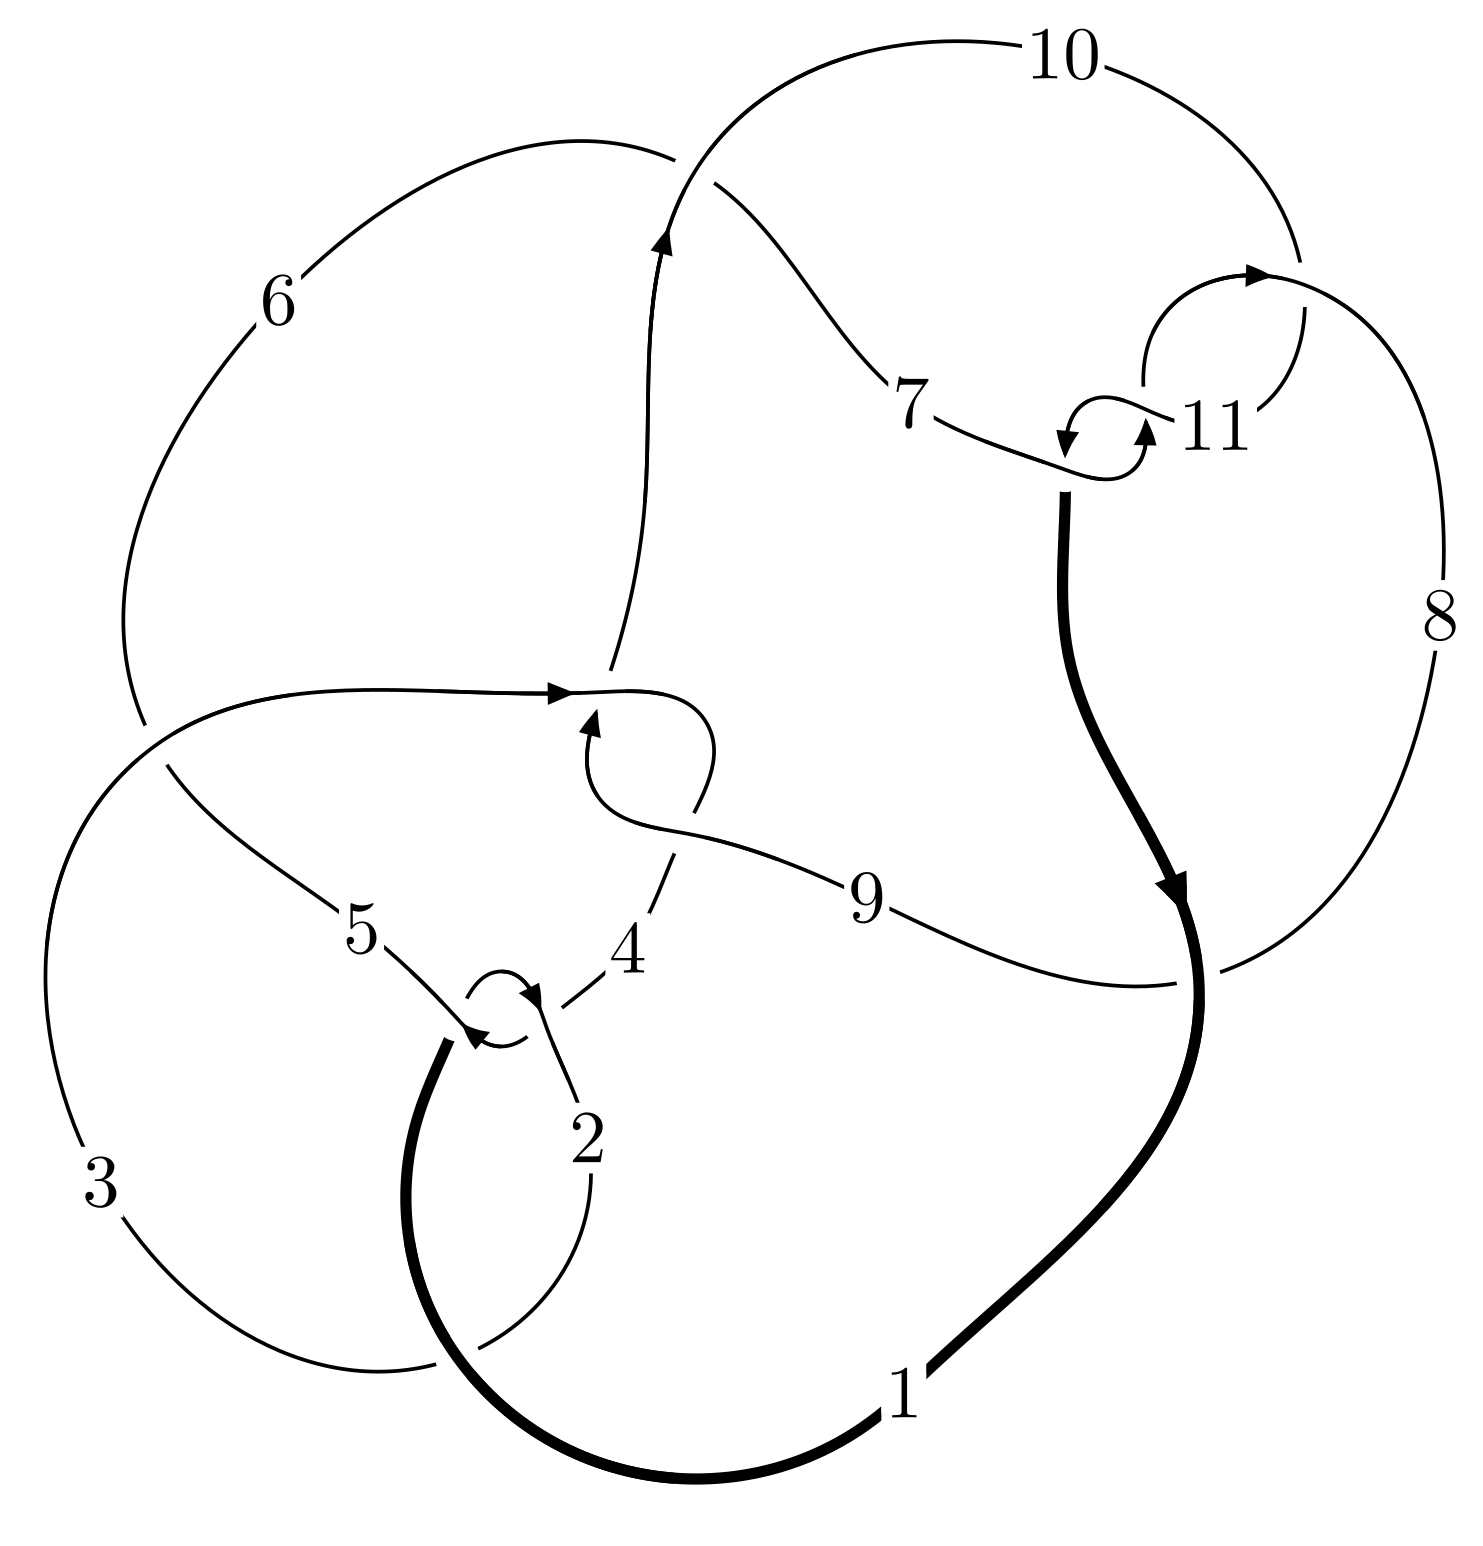
\includegraphics[width=112pt]{../../../GIT/diagram.site/Diagrams/png/636_11n_20.png}\\
\ \ \ A knot diagram\footnotemark}&
\allowdisplaybreaks
\textbf{Linearized knot diagam} \\
\cline{2-2}
 &
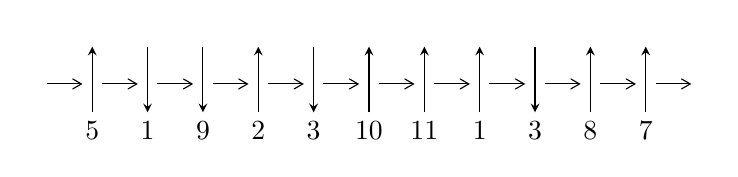
\begin{tikzpicture}[x=20pt, y=17pt]
	% nodes
	\node (C0) at (0, 0) {};
	\node (C1) at (1, 0) {};
	\node (C1U) at (1, +1) {};
	\node (C1D) at (1, -1) {5};

	\node (C2) at (2, 0) {};
	\node (C2U) at (2, +1) {};
	\node (C2D) at (2, -1) {1};

	\node (C3) at (3, 0) {};
	\node (C3U) at (3, +1) {};
	\node (C3D) at (3, -1) {9};

	\node (C4) at (4, 0) {};
	\node (C4U) at (4, +1) {};
	\node (C4D) at (4, -1) {2};

	\node (C5) at (5, 0) {};
	\node (C5U) at (5, +1) {};
	\node (C5D) at (5, -1) {3};

	\node (C6) at (6, 0) {};
	\node (C6U) at (6, +1) {};
	\node (C6D) at (6, -1) {10};

	\node (C7) at (7, 0) {};
	\node (C7U) at (7, +1) {};
	\node (C7D) at (7, -1) {11};

	\node (C8) at (8, 0) {};
	\node (C8U) at (8, +1) {};
	\node (C8D) at (8, -1) {1};

	\node (C9) at (9, 0) {};
	\node (C9U) at (9, +1) {};
	\node (C9D) at (9, -1) {3};

	\node (C10) at (10, 0) {};
	\node (C10U) at (10, +1) {};
	\node (C10D) at (10, -1) {8};

	\node (C11) at (11, 0) {};
	\node (C11U) at (11, +1) {};
	\node (C11D) at (11, -1) {7};
	\node (C12) at (12, 0) {};

	% arrows
	\draw[->,>={angle 60}]
	(C0) edge (C1) (C1) edge (C2) (C2) edge (C3) (C3) edge (C4) (C4) edge (C5) (C5) edge (C6) (C6) edge (C7) (C7) edge (C8) (C8) edge (C9) (C9) edge (C10) (C10) edge (C11) (C11) edge (C12) ;	\draw[->,>=stealth]
	(C1D) edge (C1U) (C2U) edge (C2D) (C3U) edge (C3D) (C4D) edge (C4U) (C5U) edge (C5D) (C6D) edge (C6U) (C7D) edge (C7U) (C8D) edge (C8U) (C9U) edge (C9D) (C10D) edge (C10U) (C11D) edge (C11U) ;
	\end{tikzpicture} \\
\hhline{~~} \\& 
\textbf{Solving Sequence} \\ \cline{2-2} 
 &
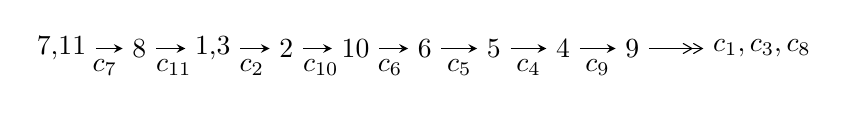
\begin{tikzpicture}[x=25pt, y=7pt]
	% node
	\node (A0) at (-1/8, 0) {7,11};
	\node (A1) at (1, 0) {8};
	\node (A2) at (33/16, 0) {1,3};
	\node (A3) at (25/8, 0) {2};
	\node (A4) at (33/8, 0) {10};
	\node (A5) at (41/8, 0) {6};
	\node (A6) at (49/8, 0) {5};
	\node (A7) at (57/8, 0) {4};
	\node (A8) at (65/8, 0) {9};
	\node (C1) at (1/2, -1) {$c_{7}$};
	\node (C2) at (3/2, -1) {$c_{11}$};
	\node (C3) at (21/8, -1) {$c_{2}$};
	\node (C4) at (29/8, -1) {$c_{10}$};
	\node (C5) at (37/8, -1) {$c_{6}$};
	\node (C6) at (45/8, -1) {$c_{5}$};
	\node (C7) at (53/8, -1) {$c_{4}$};
	\node (C8) at (61/8, -1) {$c_{9}$};
	\node (A9) at (10, 0) {$c_{1},c_{3},c_{8}$};

	% edge
	\draw[->,>=stealth]	
	(A0) edge (A1) (A1) edge (A2) (A2) edge (A3) (A3) edge (A4) (A4) edge (A5) (A5) edge (A6) (A6) edge (A7) (A7) edge (A8) ;
	\draw[->>,>={angle 60}]	
	(A8) edge (A9);
\end{tikzpicture} \\ 

\end{tabular} \\

\footnotetext{
The image of knot diagram is generated by the software ``\textbf{Draw programme}" developed by Andrew Bartholomew(\url{http://www.layer8.co.uk/maths/draw/index.htm\#Running-draw}), where we modified some parts for our purpose(\url{https://github.com/CATsTAILs/LinksPainter}).
}\phantom \\ \newline 
\centering \textbf{Ideals for irreducible components\footnotemark of $X_{\text{par}}$} 
 
\begin{align*}
I^u_{1}&=\langle 
- u^{16}+2 u^{15}+\cdots+2 b-1,\;-2 u^{16}+6 u^{15}+\cdots+2 a+5,\;u^{17}-3 u^{16}+\cdots-2 u+1\rangle \\
I^u_{2}&=\langle 
u^2 a+b+a,\;- u^2 a+a^2- a u- a- u,\;u^3+u^2+2 u+1\rangle \\
\\
\end{align*}
\raggedright * 2 irreducible components of $\dim_{\mathbb{C}}=0$, with total 23 representations.\\
\footnotetext{All coefficients of polynomials are rational numbers. But the coefficients are sometimes approximated in decimal forms when there is not enough margin.}
\newpage
\renewcommand{\arraystretch}{1}
\centering \section*{I. $I^u_{1}= \langle - u^{16}+2 u^{15}+\cdots+2 b-1,\;-2 u^{16}+6 u^{15}+\cdots+2 a+5,\;u^{17}-3 u^{16}+\cdots-2 u+1 \rangle$}
\flushleft \textbf{(i) Arc colorings}\\
\begin{tabular}{m{7pt} m{180pt} m{7pt} m{180pt} }
\flushright $a_{7}=$&$\begin{pmatrix}1\\0\end{pmatrix}$ \\
\flushright $a_{11}=$&$\begin{pmatrix}0\\u\end{pmatrix}$ \\
\flushright $a_{8}=$&$\begin{pmatrix}1\\- u^2\end{pmatrix}$ \\
\flushright $a_{1}=$&$\begin{pmatrix}u\\u\end{pmatrix}$ \\
\flushright $a_{3}=$&$\begin{pmatrix}u^{16}-3 u^{15}+\cdots+4 u-\frac{5}{2}\\\frac{1}{2} u^{16}- u^{15}+\cdots+2 u+\frac{1}{2}\end{pmatrix}$ \\
\flushright $a_{2}=$&$\begin{pmatrix}\frac{3}{2} u^{16}-\frac{9}{2} u^{15}+\cdots+\frac{11}{2} u-3\\u^{16}-\frac{5}{2} u^{15}+\cdots+12 u^3+\frac{7}{2} u\end{pmatrix}$ \\
\flushright $a_{10}=$&$\begin{pmatrix}- u\\u^3+u\end{pmatrix}$ \\
\flushright $a_{6}=$&$\begin{pmatrix}- u^4- u^2+1\\u^6+2 u^4+u^2\end{pmatrix}$ \\
\flushright $a_{5}=$&$\begin{pmatrix}\frac{1}{2} u^{14}- u^{13}+\cdots+4 u+\frac{3}{2}\\-\frac{1}{2} u^{16}+u^{15}+\cdots- u+\frac{1}{2}\end{pmatrix}$ \\
\flushright $a_{4}=$&$\begin{pmatrix}- u^{16}+5 u^{15}+\cdots-5 u+\frac{9}{2}\\-\frac{3}{2} u^{16}+5 u^{15}+\cdots-5 u+\frac{3}{2}\end{pmatrix}$ \\
\flushright $a_{9}=$&$\begin{pmatrix}- u^4- u^2+1\\- u^4-2 u^2\end{pmatrix}$\\ \flushright $a_{9}=$&$\begin{pmatrix}- u^4- u^2+1\\- u^4-2 u^2\end{pmatrix}$\\&\end{tabular}
\flushleft \textbf{(ii) Obstruction class $= -1$}\\~\\
\flushleft \textbf{(iii) Cusp Shapes $= u^{16}-\frac{3}{2} u^{15}+\frac{13}{2} u^{14}-\frac{15}{2} u^{13}+\frac{33}{2} u^{12}-19 u^{11}+23 u^{10}-\frac{67}{2} u^9+24 u^8-\frac{81}{2} u^7+22 u^6-17 u^5+12 u^4+13 u^3+\frac{19}{2} u+\frac{1}{2}$}\\~\\
\newpage\renewcommand{\arraystretch}{1}
\flushleft \textbf{(iv) u-Polynomials at the component}\newline \\
\begin{tabular}{m{50pt}|m{274pt}}
Crossings & \hspace{64pt}u-Polynomials at each crossing \\
\hline $$\begin{aligned}c_{1},c_{4}\end{aligned}$$&$\begin{aligned}
&u^{17}+4 u^{16}+\cdots+3 u+1
\end{aligned}$\\
\hline $$\begin{aligned}c_{2}\end{aligned}$$&$\begin{aligned}
&u^{17}+2 u^{16}+\cdots+3 u-1
\end{aligned}$\\
\hline $$\begin{aligned}c_{3},c_{9}\end{aligned}$$&$\begin{aligned}
&u^{17}+u^{16}+\cdots-96 u-64
\end{aligned}$\\
\hline $$\begin{aligned}c_{5}\end{aligned}$$&$\begin{aligned}
&u^{17}-4 u^{16}+\cdots+557 u+137
\end{aligned}$\\
\hline $$\begin{aligned}c_{6},c_{8}\end{aligned}$$&$\begin{aligned}
&u^{17}-3 u^{16}+\cdots+2 u-1
\end{aligned}$\\
\hline $$\begin{aligned}c_{7},c_{10},c_{11}\end{aligned}$$&$\begin{aligned}
&u^{17}+3 u^{16}+\cdots-2 u-1
\end{aligned}$\\
\hline
\end{tabular}\\~\\
\newpage\renewcommand{\arraystretch}{1}
\flushleft \textbf{(v) Riley Polynomials at the component}\newline \\
\begin{tabular}{m{50pt}|m{274pt}}
Crossings & \hspace{64pt}Riley Polynomials at each crossing \\
\hline $$\begin{aligned}c_{1},c_{4}\end{aligned}$$&$\begin{aligned}
&y^{17}+2 y^{16}+\cdots+3 y-1
\end{aligned}$\\
\hline $$\begin{aligned}c_{2}\end{aligned}$$&$\begin{aligned}
&y^{17}+30 y^{16}+\cdots+3 y-1
\end{aligned}$\\
\hline $$\begin{aligned}c_{3},c_{9}\end{aligned}$$&$\begin{aligned}
&y^{17}+35 y^{16}+\cdots+9216 y-4096
\end{aligned}$\\
\hline $$\begin{aligned}c_{5}\end{aligned}$$&$\begin{aligned}
&y^{17}+58 y^{16}+\cdots-518053 y-18769
\end{aligned}$\\
\hline $$\begin{aligned}c_{6},c_{8}\end{aligned}$$&$\begin{aligned}
&y^{17}-31 y^{16}+\cdots-14 y-1
\end{aligned}$\\
\hline $$\begin{aligned}c_{7},c_{10},c_{11}\end{aligned}$$&$\begin{aligned}
&y^{17}+13 y^{16}+\cdots-14 y-1
\end{aligned}$\\
\hline
\end{tabular}\\~\\
\newpage\flushleft \textbf{(vi) Complex Volumes and Cusp Shapes}
$$\begin{array}{c|c|c}  
\text{Solutions to }I^u_{1}& \I (\text{vol} + \sqrt{-1}CS) & \text{Cusp shape}\\
 \hline 
\begin{aligned}
u &= \phantom{-}0.219268 + 0.999289 I \\
a &= \phantom{-}1.80602 - 0.25255 I \\
b &= \phantom{-}0.77227 - 1.25221 I\end{aligned}
 & -1.31705 + 3.54605 I & \phantom{-}2.16487 - 2.95335 I \\ \hline\begin{aligned}
u &= \phantom{-}0.219268 - 0.999289 I \\
a &= \phantom{-}1.80602 + 0.25255 I \\
b &= \phantom{-}0.77227 + 1.25221 I\end{aligned}
 & -1.31705 - 3.54605 I & \phantom{-}2.16487 + 2.95335 I \\ \hline\begin{aligned}
u &= \phantom{-}1.052720 + 0.047013 I \\
a &= \phantom{-}0.092101 - 0.115408 I \\
b &= -0.02224 - 2.20267 I\end{aligned}
 & \phantom{-}15.8539 + 3.8626 I & \phantom{-}6.39661 - 2.12816 I \\ \hline\begin{aligned}
u &= \phantom{-}1.052720 - 0.047013 I \\
a &= \phantom{-}0.092101 + 0.115408 I \\
b &= -0.02224 + 2.20267 I\end{aligned}
 & \phantom{-}15.8539 - 3.8626 I & \phantom{-}6.39661 + 2.12816 I \\ \hline\begin{aligned}
u &= -0.095288 + 1.269800 I \\
a &= \phantom{-}0.670660 + 0.619159 I \\
b &= \phantom{-}0.689025 + 0.075156 I\end{aligned}
 & -4.44298 - 1.97657 I & -3.41444 + 3.62302 I \\ \hline\begin{aligned}
u &= -0.095288 - 1.269800 I \\
a &= \phantom{-}0.670660 - 0.619159 I \\
b &= \phantom{-}0.689025 - 0.075156 I\end{aligned}
 & -4.44298 + 1.97657 I & -3.41444 - 3.62302 I \\ \hline\begin{aligned}
u &= -0.228042 + 0.683004 I \\
a &= -1.181530 + 0.437561 I \\
b &= -0.295357 + 0.574121 I\end{aligned}
 & \phantom{-}0.22550 - 1.43526 I & \phantom{-}4.15937 + 3.64291 I \\ \hline\begin{aligned}
u &= -0.228042 - 0.683004 I \\
a &= -1.181530 - 0.437561 I \\
b &= -0.295357 - 0.574121 I\end{aligned}
 & \phantom{-}0.22550 + 1.43526 I & \phantom{-}4.15937 - 3.64291 I \\ \hline\begin{aligned}
u &= -0.710942\phantom{ +0.000000I} \\
a &= -0.587793\phantom{ +0.000000I} \\
b &= -0.244243\phantom{ +0.000000I}\end{aligned}
 & \phantom{-}1.69761\phantom{ +0.000000I} & \phantom{-}6.54340\phantom{ +0.000000I} \\ \hline\begin{aligned}
u &= -0.281522 + 1.323870 I \\
a &= -0.413372 + 0.348973 I \\
b &= -0.121248 + 0.378439 I\end{aligned}
 & -2.51924 - 3.59257 I & \phantom{-}1.69678 + 1.62034 I\\
 \hline 
 \end{array}$$\newpage$$\begin{array}{c|c|c}  
\text{Solutions to }I^u_{1}& \I (\text{vol} + \sqrt{-1}CS) & \text{Cusp shape}\\
 \hline 
\begin{aligned}
u &= -0.281522 - 1.323870 I \\
a &= -0.413372 - 0.348973 I \\
b &= -0.121248 - 0.378439 I\end{aligned}
 & -2.51924 + 3.59257 I & \phantom{-}1.69678 - 1.62034 I \\ \hline\begin{aligned}
u &= \phantom{-}0.55805 + 1.32231 I \\
a &= -1.54225 + 1.32872 I \\
b &= -0.28772 + 2.07576 I\end{aligned}
 & \phantom{-}11.91540 + 1.84478 I & \phantom{-}3.96952 - 0.75367 I \\ \hline\begin{aligned}
u &= \phantom{-}0.55805 - 1.32231 I \\
a &= -1.54225 - 1.32872 I \\
b &= -0.28772 - 2.07576 I\end{aligned}
 & \phantom{-}11.91540 - 1.84478 I & \phantom{-}3.96952 + 0.75367 I \\ \hline\begin{aligned}
u &= \phantom{-}0.50759 + 1.37481 I \\
a &= \phantom{-}1.54834 - 1.48310 I \\
b &= \phantom{-}0.23471 - 2.13882 I\end{aligned}
 & \phantom{-}11.4057 + 9.4106 I & \phantom{-}3.33658 - 4.76975 I \\ \hline\begin{aligned}
u &= \phantom{-}0.50759 - 1.37481 I \\
a &= \phantom{-}1.54834 + 1.48310 I \\
b &= \phantom{-}0.23471 + 2.13882 I\end{aligned}
 & \phantom{-}11.4057 - 9.4106 I & \phantom{-}3.33658 + 4.76975 I \\ \hline\begin{aligned}
u &= \phantom{-}0.122694 + 0.403191 I \\
a &= -1.68607 + 0.58270 I \\
b &= \phantom{-}0.152683 + 0.763557 I\end{aligned}
 & \phantom{-}0.106087 - 1.407490 I & \phantom{-}0.91901 + 2.91397 I \\ \hline\begin{aligned}
u &= \phantom{-}0.122694 - 0.403191 I \\
a &= -1.68607 - 0.58270 I \\
b &= \phantom{-}0.152683 - 0.763557 I\end{aligned}
 & \phantom{-}0.106087 + 1.407490 I & \phantom{-}0.91901 - 2.91397 I\\
 \hline 
 \end{array}$$\newpage\newpage\renewcommand{\arraystretch}{1}
\centering \section*{II. $I^u_{2}= \langle u^2 a+b+a,\;- u^2 a+a^2- a u- a- u,\;u^3+u^2+2 u+1 \rangle$}
\flushleft \textbf{(i) Arc colorings}\\
\begin{tabular}{m{7pt} m{180pt} m{7pt} m{180pt} }
\flushright $a_{7}=$&$\begin{pmatrix}1\\0\end{pmatrix}$ \\
\flushright $a_{11}=$&$\begin{pmatrix}0\\u\end{pmatrix}$ \\
\flushright $a_{8}=$&$\begin{pmatrix}1\\- u^2\end{pmatrix}$ \\
\flushright $a_{1}=$&$\begin{pmatrix}u\\u\end{pmatrix}$ \\
\flushright $a_{3}=$&$\begin{pmatrix}a\\- u^2 a- a\end{pmatrix}$ \\
\flushright $a_{2}=$&$\begin{pmatrix}- u^2 a- a u\\-2 u^2 a- a u-2 a\end{pmatrix}$ \\
\flushright $a_{10}=$&$\begin{pmatrix}- u\\- u^2- u-1\end{pmatrix}$ \\
\flushright $a_{6}=$&$\begin{pmatrix}- u\\- u\end{pmatrix}$ \\
\flushright $a_{5}=$&$\begin{pmatrix}- u^2+a-2 u-1\\- u^2 a- a- u+1\end{pmatrix}$ \\
\flushright $a_{4}=$&$\begin{pmatrix}a\\- u^2 a- a\end{pmatrix}$ \\
\flushright $a_{9}=$&$\begin{pmatrix}- u\\- u^2- u-1\end{pmatrix}$\\ \flushright $a_{9}=$&$\begin{pmatrix}- u\\- u^2- u-1\end{pmatrix}$\\&\end{tabular}
\flushleft \textbf{(ii) Obstruction class $= 1$}\\~\\
\flushleft \textbf{(iii) Cusp Shapes $= 4 u^2 a- a u+3 u^2+5 a+3 u+4$}\\~\\
\newpage\renewcommand{\arraystretch}{1}
\flushleft \textbf{(iv) u-Polynomials at the component}\newline \\
\begin{tabular}{m{50pt}|m{274pt}}
Crossings & \hspace{64pt}u-Polynomials at each crossing \\
\hline $$\begin{aligned}c_{1},c_{2},c_{5}\end{aligned}$$&$\begin{aligned}
&(u^2+u+1)^3
\end{aligned}$\\
\hline $$\begin{aligned}c_{3},c_{9}\end{aligned}$$&$\begin{aligned}
&u^6
\end{aligned}$\\
\hline $$\begin{aligned}c_{4}\end{aligned}$$&$\begin{aligned}
&(u^2- u+1)^3
\end{aligned}$\\
\hline $$\begin{aligned}c_{6},c_{8}\end{aligned}$$&$\begin{aligned}
&(u^3- u^2+1)^2
\end{aligned}$\\
\hline $$\begin{aligned}c_{7}\end{aligned}$$&$\begin{aligned}
&(u^3+u^2+2 u+1)^2
\end{aligned}$\\
\hline $$\begin{aligned}c_{10},c_{11}\end{aligned}$$&$\begin{aligned}
&(u^3- u^2+2 u-1)^2
\end{aligned}$\\
\hline
\end{tabular}\\~\\
\newpage\renewcommand{\arraystretch}{1}
\flushleft \textbf{(v) Riley Polynomials at the component}\newline \\
\begin{tabular}{m{50pt}|m{274pt}}
Crossings & \hspace{64pt}Riley Polynomials at each crossing \\
\hline $$\begin{aligned}c_{1},c_{2},c_{4}\\c_{5}\end{aligned}$$&$\begin{aligned}
&(y^2+y+1)^3
\end{aligned}$\\
\hline $$\begin{aligned}c_{3},c_{9}\end{aligned}$$&$\begin{aligned}
&y^6
\end{aligned}$\\
\hline $$\begin{aligned}c_{6},c_{8}\end{aligned}$$&$\begin{aligned}
&(y^3- y^2+2 y-1)^2
\end{aligned}$\\
\hline $$\begin{aligned}c_{7},c_{10},c_{11}\end{aligned}$$&$\begin{aligned}
&(y^3+3 y^2+2 y-1)^2
\end{aligned}$\\
\hline
\end{tabular}\\~\\
\newpage\flushleft \textbf{(vi) Complex Volumes and Cusp Shapes}
$$\begin{array}{c|c|c}  
\text{Solutions to }I^u_{2}& \I (\text{vol} + \sqrt{-1}CS) & \text{Cusp shape}\\
 \hline 
\begin{aligned}
u &= -0.215080 + 1.307140 I \\
a &= \phantom{-}0.206350 + 1.132320 I \\
b &= -0.500000 + 0.866025 I\end{aligned}
 & -3.02413 - 4.85801 I & -1.45566 + 6.64456 I \\ \hline\begin{aligned}
u &= -0.215080 + 1.307140 I \\
a &= -1.083790 - 0.387453 I \\
b &= -0.500000 - 0.866025 I\end{aligned}
 & -3.02413 - 0.79824 I & \phantom{-}2.09851 - 0.12339 I \\ \hline\begin{aligned}
u &= -0.215080 - 1.307140 I \\
a &= \phantom{-}0.206350 - 1.132320 I \\
b &= -0.500000 - 0.866025 I\end{aligned}
 & -3.02413 + 4.85801 I & -1.45566 - 6.64456 I \\ \hline\begin{aligned}
u &= -0.215080 - 1.307140 I \\
a &= -1.083790 + 0.387453 I \\
b &= -0.500000 + 0.866025 I\end{aligned}
 & -3.02413 + 0.79824 I & \phantom{-}2.09851 + 0.12339 I \\ \hline\begin{aligned}
u &= -0.569840\phantom{ +0.000000I} \\
a &= \phantom{-}0.377439 + 0.653743 I \\
b &= -0.500000 - 0.866025 I\end{aligned}
 & \phantom{-}1.11345 - 2.02988 I & \phantom{-}5.85715 + 4.49037 I \\ \hline\begin{aligned}
u &= -0.569840\phantom{ +0.000000I} \\
a &= \phantom{-}0.377439 - 0.653743 I \\
b &= -0.500000 + 0.866025 I\end{aligned}
 & \phantom{-}1.11345 + 2.02988 I & \phantom{-}5.85715 - 4.49037 I\\
 \hline 
 \end{array}$$\newpage
\newpage\renewcommand{\arraystretch}{1}
\centering \section*{ III. u-Polynomials}
\begin{tabular}{m{50pt}|m{274pt}}
Crossings & \hspace{64pt}u-Polynomials at each crossing \\
\hline $$\begin{aligned}c_{1}\end{aligned}$$&$\begin{aligned}
&((u^2+u+1)^3)(u^{17}+4 u^{16}+\cdots+3 u+1)
\end{aligned}$\\
\hline $$\begin{aligned}c_{2}\end{aligned}$$&$\begin{aligned}
&((u^2+u+1)^3)(u^{17}+2 u^{16}+\cdots+3 u-1)
\end{aligned}$\\
\hline $$\begin{aligned}c_{3},c_{9}\end{aligned}$$&$\begin{aligned}
&u^6(u^{17}+u^{16}+\cdots-96 u-64)
\end{aligned}$\\
\hline $$\begin{aligned}c_{4}\end{aligned}$$&$\begin{aligned}
&((u^2- u+1)^3)(u^{17}+4 u^{16}+\cdots+3 u+1)
\end{aligned}$\\
\hline $$\begin{aligned}c_{5}\end{aligned}$$&$\begin{aligned}
&((u^2+u+1)^3)(u^{17}-4 u^{16}+\cdots+557 u+137)
\end{aligned}$\\
\hline $$\begin{aligned}c_{6},c_{8}\end{aligned}$$&$\begin{aligned}
&((u^3- u^2+1)^2)(u^{17}-3 u^{16}+\cdots+2 u-1)
\end{aligned}$\\
\hline $$\begin{aligned}c_{7}\end{aligned}$$&$\begin{aligned}
&((u^3+u^2+2 u+1)^2)(u^{17}+3 u^{16}+\cdots-2 u-1)
\end{aligned}$\\
\hline $$\begin{aligned}c_{10},c_{11}\end{aligned}$$&$\begin{aligned}
&((u^3- u^2+2 u-1)^2)(u^{17}+3 u^{16}+\cdots-2 u-1)
\end{aligned}$\\
\hline
\end{tabular}\newpage\renewcommand{\arraystretch}{1}
\centering \section*{ IV. Riley Polynomials}
\begin{tabular}{m{50pt}|m{274pt}}
Crossings & \hspace{64pt}Riley Polynomials at each crossing \\
\hline $$\begin{aligned}c_{1},c_{4}\end{aligned}$$&$\begin{aligned}
&((y^2+y+1)^3)(y^{17}+2 y^{16}+\cdots+3 y-1)
\end{aligned}$\\
\hline $$\begin{aligned}c_{2}\end{aligned}$$&$\begin{aligned}
&((y^2+y+1)^3)(y^{17}+30 y^{16}+\cdots+3 y-1)
\end{aligned}$\\
\hline $$\begin{aligned}c_{3},c_{9}\end{aligned}$$&$\begin{aligned}
&y^6(y^{17}+35 y^{16}+\cdots+9216 y-4096)
\end{aligned}$\\
\hline $$\begin{aligned}c_{5}\end{aligned}$$&$\begin{aligned}
&((y^2+y+1)^3)(y^{17}+58 y^{16}+\cdots-518053 y-18769)
\end{aligned}$\\
\hline $$\begin{aligned}c_{6},c_{8}\end{aligned}$$&$\begin{aligned}
&((y^3- y^2+2 y-1)^2)(y^{17}-31 y^{16}+\cdots-14 y-1)
\end{aligned}$\\
\hline $$\begin{aligned}c_{7},c_{10},c_{11}\end{aligned}$$&$\begin{aligned}
&((y^3+3 y^2+2 y-1)^2)(y^{17}+13 y^{16}+\cdots-14 y-1)
\end{aligned}$\\
\hline
\end{tabular}
\vskip 2pc
\end{document}